\documentclass[conference,a4paper]{IEEEtran}
\IEEEoverridecommandlockouts

\usepackage[utf8]{inputenc}
\usepackage[T1]{fontenc}
\usepackage[spanish,es-noshorthands,es-tabla]{babel}
\usepackage{cite}
\usepackage{amsmath,amssymb}
\usepackage{graphicx}
\usepackage{booktabs}
\usepackage{multirow}
\usepackage{url}
\usepackage[hidelinks]{hyperref}
\usepackage{xcolor}
\decimalpoint

\begin{document}

\title{Lectura de cartas y control por gestos para Blackjack con visión por computadora:\\
de datos sintéticos a una mesa real}

\author{\IEEEauthorblockN{Cristhian Pettico, Rodolfo Di Chiazza, Julian Blanco}
\IEEEauthorblockA{Carrera de Especialización en Inteligencia Artificial (CEIA)\\
Facultad de Ingeniería, Universidad de Buenos Aires\\
Buenos Aires, Argentina}}

\maketitle

\begin{abstract}
Presentamos un prototipo que permite jugar al Blackjack sobre una mesa real: una cámara cenital reconoce las cartas
que se reparten y el jugador pide carta o se planta con gestos de la mano. Comparamos dos estrategias para reconocer el
índice de la esquina de cada carta: un detector YOLO11 de 13 clases (A) y un detector de una clase seguido de una
ResNet-18 (B). Ambas alcanzan mAP50 $\approx$ 0,99 en el dataset sintético de entrenamiento, pero sobre fotos reales
caen a 0,68--0,86. El ajuste fino con fotos de otro mazo casi no se transfiere (F1 de 0,78 a 0,78
en A y a 0,83 en B), mientras que con 79 cuadros del escenario propio el recall de A sube de 0,66 a 0,96 (F1 0,96). Evaluamos la robustez ante rotación, oclusión,
iluminación y fondo: la oclusión es la perturbación más dañina, la iluminación afecta mucho más en datos reales que en
sintéticos y el fondo casi no influye. El sistema completo (emparejamiento geométrico de esquinas, seguimiento
ByteTrack, gestos con MediaPipe y un motor de reglas) resolvió correctamente las 4 partidas reales registradas.
\end{abstract}

\begin{IEEEkeywords}
detección de objetos, YOLO11, brecha sintético--real, robustez, seguimiento, gestos de la mano, Blackjack
\end{IEEEkeywords}

% =====================================================================================================================
\section{Introducción}

Las mesas de juego de los casinos se supervisan con cámaras para registrar las manos, detectar errores del crupier y
conductas como el conteo de cartas. Automatizar esa lectura es un problema clásico de visión por computadora: Zutis y
Hoey \cite{zutis2009} monitorearon partidas de Blackjack con una cámara estéreo cenital usando descriptores clásicos, y
trabajos recientes integran el reconocimiento de cartas con la recomendación de la estrategia básica
\cite{gupta2024} o entrenan detectores YOLO sobre datasets sintéticos y reales de cartas \cite{kostadinov2024}. El
problema es en apariencia simple ---52 clases bien definidas---, pero en una mesa real las cartas aparecen giradas,
superpuestas, tapadas por las manos y bajo iluminación variable.

El \textbf{objetivo} de este trabajo es entrenar un detector de cartas y \textbf{evaluar experimentalmente su
desempeño} ante rotaciones, oclusiones, cambios de iluminación y de fondo, e integrarlo en una aplicación que permita
jugar Blackjack en una mesa real. Como en Blackjack el palo no influye en el puntaje, el reconocimiento se limita a
los 13 valores. Las contribuciones son:
\begin{itemize}
\item Una comparación entre un detector de un paso (A) y uno de dos etapas (B), en precisión y latencia, sobre datos
sintéticos, un dataset real público y un dataset real propio.
\item La cuantificación de la brecha sintético--real y de cuándo el ajuste fino con fotos reales la cierra.
\item Un estudio de robustez ante 5 familias de perturbaciones y un análisis de las confusiones entre valores.
\item Un sistema completo y reproducible ---cartas, seguimiento, gestos y reglas--- validado con partidas reales.
\end{itemize}

% =====================================================================================================================
\section{Metodología}

\begin{figure*}[t]
\centering
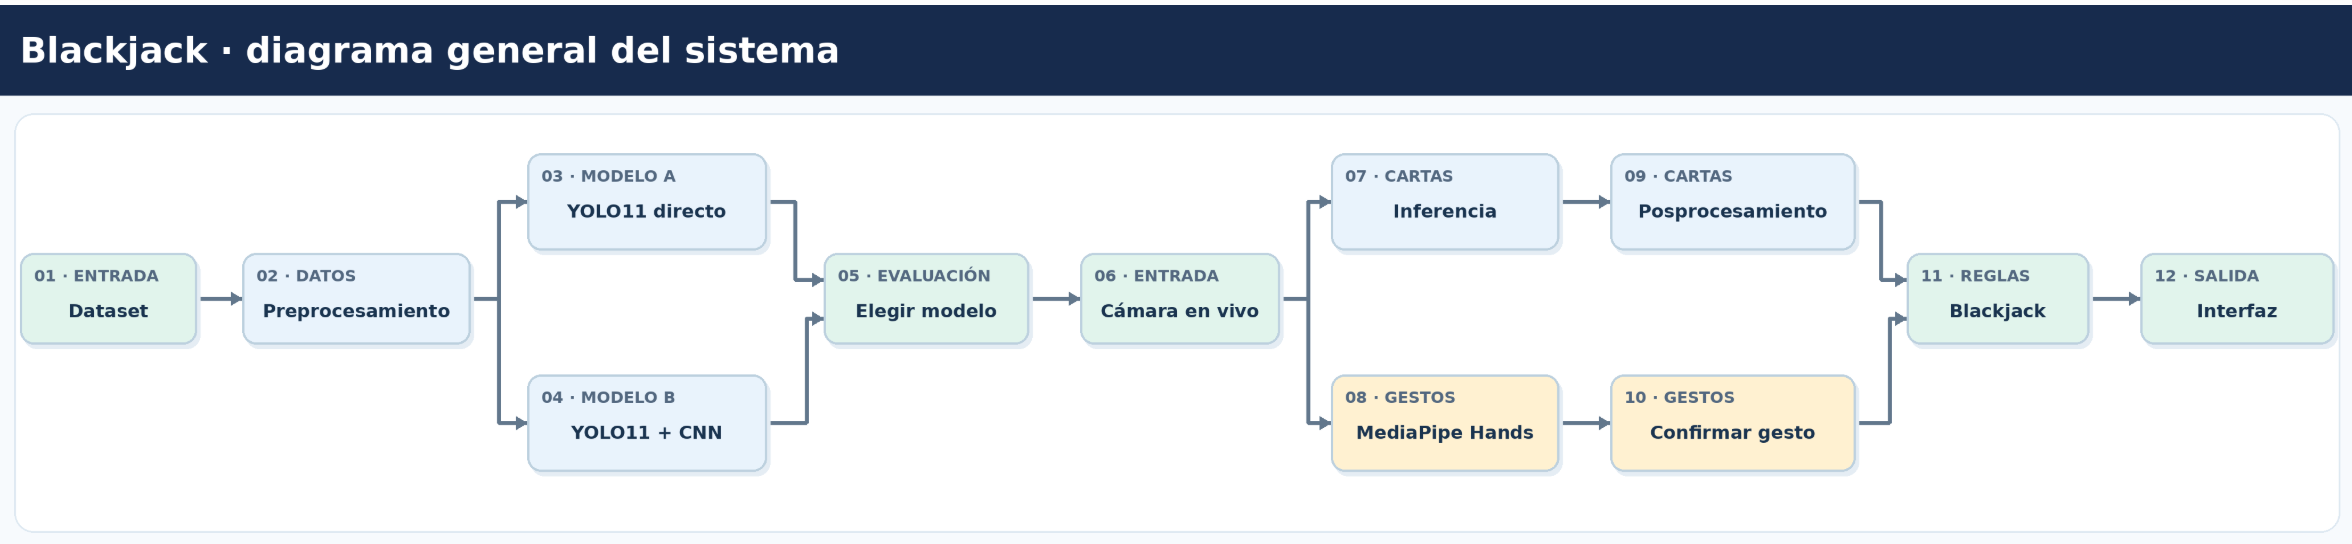
\includegraphics[width=\textwidth]{figuras/arquitectura.png}
\caption{Arquitectura del sistema. Fuera de línea se entrenan los modelos A y B y se elige uno (bloques 01--05); en
línea, cada cuadro de la cámara pasa por la inferencia de cartas y por MediaPipe, y ambas salidas alimentan el motor
de reglas y la interfaz (bloques 06--12).}
\label{fig:arquitectura}
\end{figure*}

La Fig.~\ref{fig:arquitectura} resume el sistema. Los modelos no detectan la carta entera sino el \textbf{índice de
la esquina} (valor y palo impresos), que es lo único legible cuando las cartas se superponen.

\subsection{Datos}
\textbf{Sintético.} 10.100 imágenes de 512$\times$512 (7.070 / 2.020 / 1.010) derivadas del dataset \emph{Playing
Cards} de Roboflow \cite{roboflowcards}: cartas generadas y pegadas sobre fondos texturados, con las etiquetas
reducidas a 13 valores (A) o a una clase (B). Para la CNN de B se recortaron las cajas con un margen del 10\%
(28.280 / 8.080 / 4.040 recortes).
\textbf{Real público.} 98 fotos de 416$\times$416 (69 / 18 / 11) de \cite{kostadinov2024}: un solo palo (corazones) y
un mazo con índices en las cuatro esquinas.
\textbf{Real propio.} Para el escenario de la demo se grabaron 4 sesiones con la cámara del juego (un celular cenital)
y se extrajeron 130 cuadros (79 / 21 / 30) que se pre-etiquetaron con el modelo A y se corrigieron a mano: 1.688
esquinas, con muchas cartas superpuestas. Los conjuntos se separaron \emph{por sesión}, para que cuadros casi iguales
no queden en entrenamiento y prueba.

\subsection{Modelos}
\textbf{A (un paso):} YOLO11s \cite{ultralytics2024,khanam2024} preentrenado en COCO, ajustado para 13 clases (640
px, 50 épocas). Se eligió YOLO11 por su balance entre precisión y latencia en CPU y porque integra seguimiento.
\textbf{B (dos etapas):} el mismo YOLO11s con una sola clase localiza las esquinas, se recortan con el mismo margen y
una ResNet-18 \cite{he2016} preentrenada en ImageNet clasifica el valor (96$\times$96, sin volteos porque un índice
espejado no es una carta válida). La hipótesis de B es que separar ``dónde'' de ``qué'' facilita cada tarea.
\textbf{Ajuste fino con fotos reales:} en cada época se mezclan 400 imágenes sintéticas con el entrenamiento real
repetido 5 veces, y el mejor modelo se elige con la validación real; el test real no se usa hasta la evaluación.
Se ajustó por separado con el dataset público y con el propio. En adelante, A \emph{base} y B \emph{base}
son los modelos entrenados solo con datos sintéticos; A \emph{ft} y B \emph{ft}, los ajustados con el dataset
público, y A \emph{propio} y B \emph{propio}, los ajustados con el dataset propio.

\subsection{De esquinas a cartas y a la partida}
\textbf{Emparejamiento.} Las dos esquinas de una carta están en vértices opuestos. Un par se acepta si la distancia
entre centros, relativa al lado mayor de las cajas, está en $[3{,}3;\,4{,}8]$ y el ángulo de la diagonal es cercano
a 50° (carta vertical) o 140° (carta girada 90°). La ventana se calibró con las esquinas etiquetadas del dataset
propio; usar el lado mayor y no la raíz del área la hace robusta a cartas giradas. Los pares se eligen de menor a mayor
costo sin reutilizar esquinas, y una esquina sin pareja cuenta como carta (la otra puede estar tapada). Se descartan
duplicados (supresión no máxima agnóstica a la clase, esquinas superpuestas del mismo valor) e índices ``imposibles''
dentro de una carta del mismo valor.
\textbf{Seguimiento.} ByteTrack \cite{zhang2022bytetrack} asigna a cada esquina un identificador; su valor se decide
por votación ponderada en 15 cuadros, una esquina perdida se recuerda 10 cuadros y la mano mostrada es la mediana, por
valor, de los últimos 15 cuadros.
\textbf{Gestos.} MediaPipe Hands \cite{zhang2020mediapipe} da 21 puntos por mano; la pose se clasifica con cocientes
de distancias muñeca--punta / muñeca--nudillo, invariantes a la rotación y la escala: \emph{apuntar} (solo el índice
extendido, sostenido 0,5~s) pide carta y la \emph{palma} abierta (sostenida 1,2~s o desplazada) se planta.
\textbf{Reglas.} Un motor de estados (reparto, jugador, casa, fin) toma la mano estabilizada como fuente válida: la
Casa pide hasta llegar a 17, el As vale 11 si no se pasa de 21, y un cambio se acepta tras 5 cuadros estables (20 si agrega
cartas que nadie pidió). Mientras hay una mano sobre la mesa no se confirma ningún cambio.

\subsection{Protocolo de evaluación}
Una detección es correcta si su IoU (Intersection over Union) con una esquina real es $\geq 0{,}5$ y el valor coincide. Se reportan mAP50
(promedio de los 13 valores), precisión (P), recall (R) y F1 con confianza $\geq 0{,}5$, y la latencia por imagen en
CPU (AMD Ryzen 7 7840U).

\textbf{Robustez.} Sobre el test propio (30 cuadros, 412 esquinas) y una muestra fija de 100 imágenes del test
sintético se aplican 26 condiciones en 5 perturbaciones (Fig.~\ref{fig:perturbaciones}): rotación alrededor del
centro (15° a 180°, 6 niveles), oclusión de cada índice con un rectángulo desde un borde al azar (10\% a 60\% del
índice, 6 niveles), brillo (ganancia $\times$0,2 a $\times$2,5, 6 niveles), contraste (factor $\times$0,6 a
$\times$0,15, 4 niveles) y sombra (gradiente de luz con mínimo del 60\% al 10\%, 4 niveles). Todas las configuraciones
ven exactamente la misma imagen perturbada (semilla fija) y, al rotar, las cajas reales se transforman junto con la
imagen. Para el \textbf{fondo}, reemplazar el fondo de una foto con una máscara de color no resultó confiable, por lo
que se compusieron 30 escenas con 7 cartas reales recortadas del mazo de la demo (6 valores, 244 esquinas) sobre 8
fondos, con las mismas cartas y posiciones en todos: así solo cambia el fondo.
\textbf{Confusiones.} Cada esquina real se cruza con la detección que más se le superpone (IoU $\geq$ 0,5, sin mirar
el valor), lo que separa tres errores: valor equivocado, esquina no detectada y falso positivo.

\begin{figure*}[t]
\centering
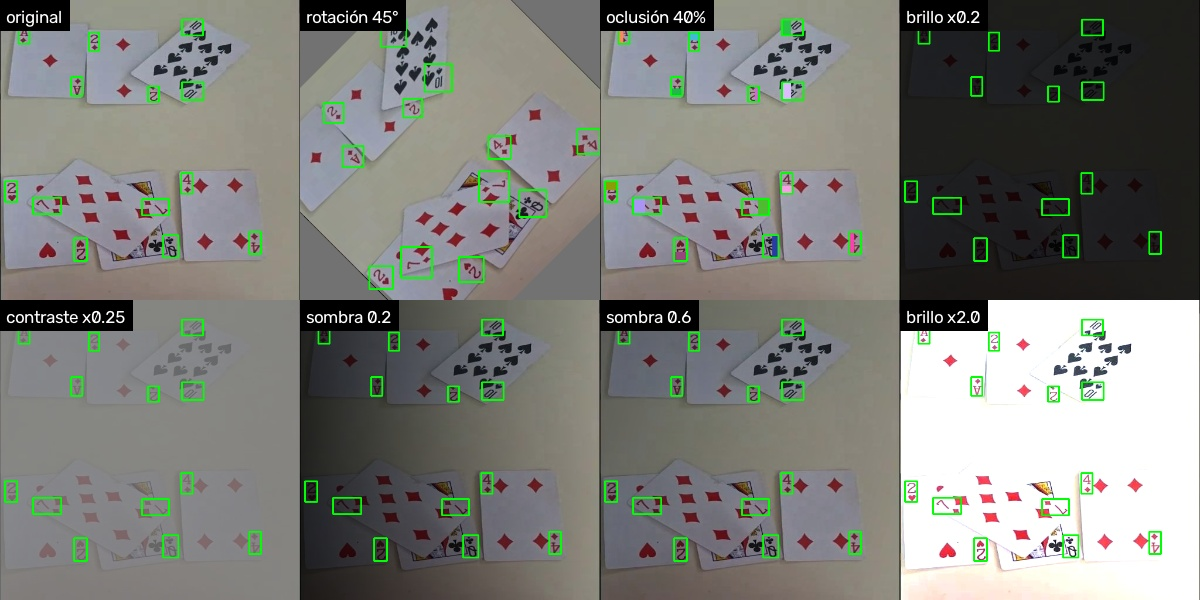
\includegraphics[width=0.86\textwidth]{figuras/perturbaciones.jpg}
\caption{Ejemplos de perturbaciones sobre un cuadro del test propio, con las esquinas reales en verde: rotación,
oclusión del índice (rectángulo de color desde un borde), brillo, contraste y sombra (gradiente de luz; el valor
indica la luz mínima). Cada familia se evalúa en varios niveles de severidad (Fig.~\ref{fig:robustez}).}
\label{fig:perturbaciones}
\end{figure*}

% =====================================================================================================================
\section{Resultados}

\subsection{Brecha sintético--real y ajuste fino}

\begin{table}[t]
\centering
\caption{Desempeño por esquina (IoU $\geq$ 0,5 y valor correcto) en los tres dominios. \emph{ft}: ajustado con el
dataset real público; \emph{propio}: ajustado con el dataset propio. Latencia en CPU sobre el test propio.}
\label{tab:dominios}
\setlength{\tabcolsep}{3.2pt}
\begin{tabular}{lcccccc}
\toprule
 & \multicolumn{2}{c}{Sintético} & \multicolumn{2}{c}{Real público} & \multicolumn{2}{c}{Real propio} \\
\cmidrule(lr){2-3}\cmidrule(lr){4-5}\cmidrule(lr){6-7}
Modelo & mAP50 & F1 & mAP50 & F1 & mAP50 & F1 \\
\midrule
A base       & 0,995 & 1,00 & 0,68 & 0,72 & 0,86 & 0,78 \\
B base       & 0,995$^\dagger$ & 1,00 & 0,68 & 0,72 & 0,82 & 0,78 \\
A \emph{ft}     & --    & --   & \textbf{0,89} & \textbf{0,89} & 0,86 & 0,78 \\
B \emph{ft}     & --    & --   & 0,77 & 0,78 & 0,90 & 0,83 \\
A \emph{propio} & --    & --   & 0,70 & 0,71 & \textbf{0,98} & \textbf{0,96} \\
B \emph{propio} & --    & --   & 0,75 & 0,73 & 0,94 & 0,93 \\
\midrule
\multicolumn{7}{l}{Latencia (ms/imagen): A 100--114; B 136--143} \\
\bottomrule
\multicolumn{7}{l}{\footnotesize $^\dagger$Detector de B; la CNN alcanza 100\% de exactitud en el test sintético.}
\end{tabular}
\end{table}

La Tabla~\ref{tab:dominios} muestra el resultado central. En el dominio sintético el problema está prácticamente
resuelto (mAP50 0,995 y 100\% de exactitud de la CNN), pero el desempeño \textbf{cae a 0,68--0,86 de mAP50 en fotos
reales}, una brecha conocida en el entrenamiento con datos sintéticos \cite{tremblay2018}. El ajuste fino la cierra,
pero \textbf{sobre todo en su propio dominio}: A \emph{ft} sube a F1 0,89 en el dataset público y queda igual que A base
(0,78) en el escenario propio, y A \emph{propio}, ajustado con 79 cuadros propios, llega a F1 0,96 en su escenario
y queda igual que A base (0,71) en el público. B \emph{ft} es la excepción parcial: en el escenario
propio sube de 0,78 a 0,83, porque el ajuste mejora sobre todo a su detector de una clase, y localizar una esquina
generaliza mejor entre mazos que clasificar su valor. Aun así queda lejos de lo que se logra con fotos propias
(0,93--0,96). Para un sistema desplegado, conviene invertir en pocas fotos del escenario real antes que en más datos
genéricos.

En el escenario propio A supera a B (F1 0,96 de A \emph{propio} frente a 0,93 de B \emph{propio}) y es entre 20 y 40~ms más rápido. En el dataset
público, A y B quedan parejos en sus versiones \emph{base} y \emph{propio} (diferencias $\leq$ 0,02), y A \emph{ft}
supera a B \emph{ft} (0,89 frente a 0,78). La ventaja de B se limita a una precisión ligeramente
mayor de B base (0,99 frente a 0,96 de A base). Por eso la aplicación usa A \emph{propio}.

\subsection{Robustez}

\begin{figure*}[t]
\centering
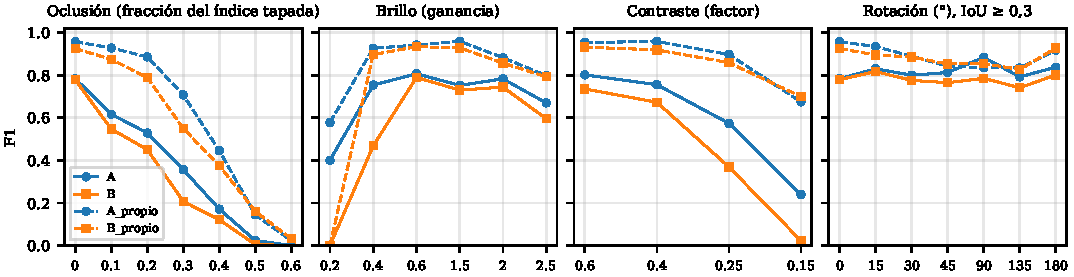
\includegraphics[width=\textwidth]{figuras/robustez.pdf}
\caption{F1 en el test propio en función de la severidad de cada perturbación (trazo lleno: A y B \emph{base}; trazo
cortado: A y B \emph{propio}). Las rotaciones se miden con IoU $\geq$ 0,3 (ver texto).}
\label{fig:robustez}
\end{figure*}

\begin{table}[t]
\centering
\caption{F1 medio por familia de perturbación (promedio de sus niveles; IoU $\geq$ 0,5). Sin perturbar, el F1 es
0,78 / 0,78 / 0,96 / 0,93 en el test propio y 1,00 en el sintético.}
\label{tab:robustez}
\setlength{\tabcolsep}{4pt}
\begin{tabular}{llcccc}
\toprule
Dominio & Familia & A & B & A \emph{propio} & B \emph{propio} \\
\midrule
\multirow{3}{*}{Real propio} & Rotación & 0,76 & 0,72 & \textbf{0,81} & 0,80 \\
 & Oclusión    & 0,28 & 0,22 & \textbf{0,52} & 0,46 \\
 & Iluminación & 0,69 & 0,58 & \textbf{0,88} & 0,82 \\
\midrule
\multirow{3}{*}{Sintético} & Rotación & 0,74 & 0,72 & 0,74 & 0,71 \\
 & Oclusión    & \textbf{0,74} & 0,63 & 0,72 & 0,61 \\
 & Iluminación & \textbf{0,99} & 0,98 & 0,99 & 0,98 \\
\bottomrule
\end{tabular}
\end{table}

\begin{table}[t]
\centering
\caption{F1 en niveles seleccionados de cada perturbación: test propio (4 configuraciones) y test sintético
(modelo A base); \emph{pr.}: \emph{propio}. La serie completa está en la Fig.~\ref{fig:robustez}.}
\label{tab:niveles}
\setlength{\tabcolsep}{3.5pt}
\begin{tabular}{llccccc}
\toprule
 & & \multicolumn{4}{c}{Real propio} & Sint. \\
\cmidrule(lr){3-6}\cmidrule(lr){7-7}
Perturbación & Nivel & A & B & A \emph{pr.} & B \emph{pr.} & A \\
\midrule
Ninguna    & --             & 0,78 & 0,78 & 0,96 & 0,93 & 1,00 \\
\midrule
Oclusión   & 10\%           & 0,62 & 0,55 & 0,93 & 0,87 & 1,00 \\
           & 20\%           & 0,53 & 0,45 & 0,89 & 0,79 & 1,00 \\
           & 30\%           & 0,36 & 0,21 & 0,71 & 0,55 & 0,95 \\
           & 50\%           & 0,02 & 0,00 & 0,14 & 0,16 & 0,52 \\
\midrule
Brillo     & $\times$0,2    & 0,40 & 0,00 & 0,58 & 0,00 & 1,00 \\
           & $\times$2,5    & 0,67 & 0,60 & 0,80 & 0,79 & 0,86 \\
Contraste  & $\times$0,15   & 0,24 & 0,02 & 0,67 & 0,70 & 0,99 \\
Sombra     & mín. 10\%      & 0,76 & 0,64 & 0,92 & 0,85 & 1,00 \\
\midrule
Rotación   & 45°, IoU 0,5   & 0,67 & 0,64 & 0,72 & 0,69 & 0,46 \\
(IoU 0,3   & 45°            & 0,81 & 0,76 & 0,84 & 0,85 & 0,98 \\
salvo      & 90°            & 0,88 & 0,79 & 0,84 & 0,85 & 1,00 \\
indicado)  & 180°           & 0,84 & 0,80 & 0,92 & 0,93 & 1,00 \\
\bottomrule
\end{tabular}
\end{table}

\begin{table}[t]
\centering
\caption{F1 sobre escenas compuestas con 7 cartas reales y 8 fondos (las mismas cartas y posiciones en todos).}
\label{tab:fondo}
\setlength{\tabcolsep}{2.6pt}
\begin{tabular}{lcccccccc}
\toprule
 & Mad. & Verde & Osc. & Blanco & Text. & Desor. & Ruido & Márm. \\
\midrule
A               & 0,99 & 1,00 & 1,00 & 0,99 & 1,00 & 1,00 & 0,99 & 1,00 \\
B               & 0,98 & 0,99 & 0,99 & \textbf{0,90} & 0,97 & 0,97 & 0,98 & 0,99 \\
A \emph{propio} & 0,99 & 0,99 & 0,99 & 0,98 & 0,99 & 0,99 & 0,99 & 0,99 \\
B \emph{propio} & 1,00 & 1,00 & 1,00 & 1,00 & 1,00 & 1,00 & 0,99 & 1,00 \\
\bottomrule
\end{tabular}
\end{table}

La Tabla~\ref{tab:robustez} resume cada familia y la Tabla~\ref{tab:niveles} da los niveles que se citan a
continuación; la Fig.~\ref{fig:robustez} muestra la serie completa.
\textbf{Oclusión.} Es la perturbación más dañina. En el sintético, A tolera el 30\% del índice tapado (F1 0,95) y con
el 50\% cae a 0,52. En datos reales, donde las mesas ya tienen cartas superpuestas, A base pierde desde el
10\% (0,62), mientras que A \emph{propio} resiste hasta el 20\% (0,89). Esto motivó contar como carta una esquina suelta,
la memoria del seguimiento y congelar la mesa mientras hay una mano encima.
\textbf{Iluminación.} En el sintético los modelos son casi inmunes (F1 medio $\geq$ 0,98, porque ese dataset ya
incluye variaciones de brillo); solo la sobreexposición $\times$2,5 baja A a 0,86. En datos reales, la subexposición
y el bajo contraste son críticos: con brillo $\times$0,2, B obtiene F1 0 (B base y B \emph{propio}) y A \emph{propio}
0,58; con contraste $\times$0,15, A base cae a 0,24 y A \emph{propio} mantiene 0,67. Las sombras afectan poco, salvo
a B base. El ajuste con fotos propias mejora la robustez de A a la iluminación de 0,69 (A base) a 0,88
(A \emph{propio}) de F1 medio.
\textbf{Rotación.} Con IoU $\geq$ 0,5, el F1 de A cae a 0,46 a 45° incluso en el sintético, pero es un efecto de la
medición: la caja real rotada es la caja alineada que contiene al índice girado, más grande que la predicción. Con
IoU $\geq$ 0,3, el sintético da F1 $\geq$ 0,96 en todos los ángulos. En datos reales queda una caída genuina: A
\emph{propio} pasa de 0,96 a 0,84 tanto a 45° como a 90°, y casi no pierde a 180° (0,92). La caída a 90° coincide con que
todas las fotos propias se grabaron con la cámara en una sola orientación.
\textbf{Fondo.} Con las escenas compuestas (Tabla~\ref{tab:fondo}), A obtiene F1 $\geq$ 0,99 en los 8 fondos; el
único que afecta es el blanco para B base (0,90), cuyo detector encuentra solo el 83\% de las esquinas. Con cartas
separadas, el fondo no es la dificultad: lo son la superposición y la oclusión.

\subsection{Confusiones}

\begin{table}[t]
\centering
\caption{Errores por esquina en el test propio (412 esquinas reales). \emph{Peor valor}: el valor con menor
proporción de esquinas detectadas, entre paréntesis.}
\label{tab:confusiones}
\setlength{\tabcolsep}{2.5pt}
\begin{tabular}{lcccccc}
\toprule
 & Bien & \begin{tabular}[c]{@{}c@{}}Valor\\ equiv.\end{tabular} & \begin{tabular}[c]{@{}c@{}}No\\ detect.\end{tabular}
 & \begin{tabular}[c]{@{}c@{}}Falsos\\ posit.\end{tabular} & \begin{tabular}[c]{@{}c@{}}Confusión\\ más frec.\end{tabular}
 & \begin{tabular}[c]{@{}c@{}}Peor\\ valor\end{tabular} \\
\midrule
A               & 66,3\% & 1,7\% & \textbf{32,0\%} & 5  & 8$\to$6 (5) & 9 (32\%) \\
B               & 64,1\% & 0,2\% & \textbf{35,7\%} & 1  & A$\to$4 (1) & 5 (27\%) \\
A \emph{propio} & \textbf{95,6\%} & \textbf{0\%} & 4,4\% & 17 & ninguna & 8 (58\%) \\
B \emph{propio} & 93,0\% & 2,2\% & 4,9\% & 24 & 5$\to$3 (5) & 8 (65\%) \\
\bottomrule
\end{tabular}
\end{table}

La Tabla~\ref{tab:confusiones} muestra que en el test propio casi no se confunden valores: el error dominante es no
encontrar la esquina (32\% en A base). A \emph{propio} reduce las esquinas no detectadas al 4,4\% sin introducir
confusiones, a costa de algunos falsos positivos más (17 en 412). Las confusiones que quedan son entre formas
parecidas (8$\to$6 en A base; 5$\to$3 y 8$\to$Q en B \emph{propio}, que clasifica un recorte sin contexto). Desglosando
por valor las esquinas no detectadas (columna \emph{Peor valor}), en A \emph{propio} y B \emph{propio} se concentran en el
8: A \emph{propio} no encuentra 13 de los 31 índices de 8 del test (detecta el 58\%), y esas 13 son la mayoría de sus 18
esquinas perdidas; en todos los demás valores detecta el 86\% o más. B \emph{propio} muestra el mismo patrón (11 de sus 20
esquinas perdidas son 8).

\subsection{Sistema completo}

\begin{figure}[t]
\centering
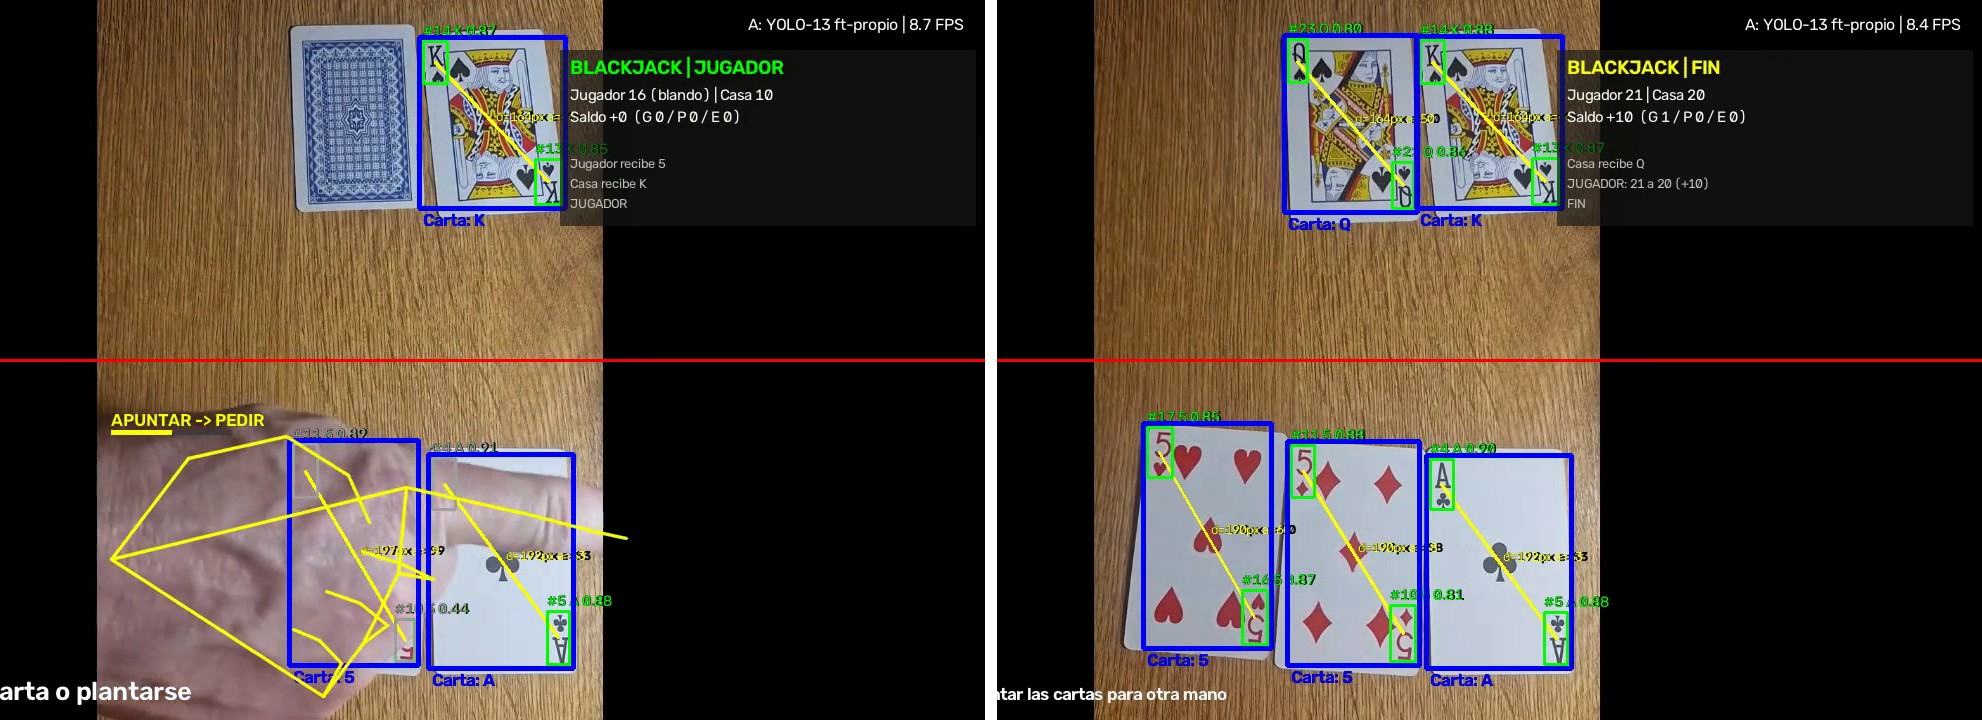
\includegraphics[width=\columnwidth]{figuras/aplicacion.jpg}
\caption{Partida real. Izquierda: el gesto \emph{apuntar} pide carta (A + 5 = 16). Derecha: el jugador llega a 21 con
un 5 girado y gana 21 a 20 (panel: etapa, puntajes, saldo y eventos).}
\label{fig:aplicacion}
\end{figure}

\textbf{Seguimiento.} En 4 videos con movimiento de cámara simulado, el seguimiento elevó la mano mostrada correcta de
50,5\% a 76,2\% y redujo los cambios de mano en 10~s de 47 a 4.
\textbf{Gestos.} Sobre fotos reales de HaGRID \cite{kapitanov2024hagrid}, la regla propuesta reconoce \emph{apuntar}
y \emph{palma} con recall 0,80 y 0,89 tanto a 0° como a 90° y 180°, mientras que el reconocedor de gestos de MediaPipe cae a 0
con la mano girada 90° o 180°, situación habitual con una cámara cenital. En clips de video, \emph{palma} se reconoce
en el 82--87\% de los casos con 4,2\% de disparos falsos.
\textbf{Partidas reales.} Se grabaron 4 partidas completas (2 ganadas por el jugador y 2 por la Casa, incluyendo un
As que pasa de 11 a 1 y una carta girada). Reproducidas cuadro a cuadro, el sistema obtiene en las 4 el mismo
resultado, cartas y gestos que se vieron en vivo, sin irregularidades (Fig.~\ref{fig:aplicacion}); el prototipo corre a
7--10 cuadros por segundo en CPU. Estas partidas quedan como prueba de regresión del sistema.

% =====================================================================================================================
\section{Conclusiones}
\begin{enumerate}
\item El rendimiento en el dataset sintético (mAP50 0,995) no anticipa el rendimiento real (0,68--0,86): evaluar con
fotos del escenario de uso es imprescindible.
\item El ajuste fino con datos reales mejora sobre todo el dominio con el que se hace: 79 cuadros del escenario
propio llevaron el recall de A de 0,66 a 0,96, mientras que fotos de otro mazo no mejoraron a A (A \emph{ft}) y solo
mejoraron parcialmente a B (B \emph{ft}: F1 de 0,78 a 0,83), a través de su detector.
\item En el escenario de uso, el detector de un paso (A) superó al de dos etapas (B) en exactitud y latencia: el contexto que ve el detector
ayuda a distinguir valores parecidos, mientras que la CNN de B clasifica un recorte aislado.
\item En datos reales el error dominante no es confundir valores sino no encontrar la esquina; la oclusión es la
perturbación más dañina y la iluminación pesa mucho más que en los datos sintéticos.
\item El fondo casi no influye, y la caída aparente ante rotaciones oblicuas se explica en gran parte por la métrica
(IoU de cajas alineadas); conviene reportar ambos umbrales.
\item La lógica de posprocesamiento ---emparejamiento geométrico, NMS agnóstico, seguimiento y congelar la mesa con
una mano encima--- fue decisiva para pasar de detecciones por cuadro a manos correctas en partidas reales.
\item Para gestos con cámara cenital, reglas invariantes a la rotación sobre los puntos de MediaPipe funcionan donde el
clasificador preentrenado falla.
\end{enumerate}
\textbf{Trabajo futuro:} reconocer el palo (permitiría detectar cartas duplicadas, imposibles con un solo mazo),
entrenar con la cámara en ambas orientaciones, más mesas e iluminaciones en el test propio y varios jugadores.
El código, los modelos, los datos y las partidas reales están disponibles en
\url{https://github.com/dichiazzar/Vision_Computadora_2_TP_2}.

\bibliographystyle{IEEEtran}
\bibliography{referencias}

\end{document}
